\documentclass{instructions}

\usepackage{alltt}
\usepackage{xspace}

\newcommand{\git}{\texttt{git}\xspace}
\newcommand\bs{\char`\\}

\graphicspath{{figs/}}

\title{Robotic Arm Mini-project\newline Part 1 -- Servo motors}
\date{\today}

\summary{
We now start the Robotic Arm mini-project. It will last until Christmas. Over
the coming 6 labs, you will design your own robotic arm (with at least 2 degrees
of freedom, but you can add more), program it with ROS, build a 3D visualisation
for it, and, if time permit, use a 3D motion planner to control it
automatically!

During this first part of the Robotic Arm project, you will learn how to control
servo motors with the Arduino Uno.
}

\objectives{
At the end of this lab, you should:

\begin{itemize}
    \item Know how to wire a servo-motor onto an Arduino board
    \item Know how to control a servo-motor with PWM signals
    \item Understand the torque characteristics of the servo-motor
\end{itemize}
}

\challenges{

    \begin{itemize}
        \item This is the first part of a six-weeks long mini-project. Plan
            ahead!
    \end{itemize}
}

\begin{document}

\maketitle


\note{
    As usual, \textbf{document in your lab journal your findings}.
Add \textbf{code snippets}, \textbf{screenshots}, \textbf{pictures} and link to \textbf{videos} as needed.

\vspace{1em}

And do not forget: \textbf{write your lab journal as a text file using the Markdown
syntax} and \textbf{push your journal and the pictures on GitHub}.

}

%%%%%%%%%%%%%%%%%%%%%%%%%%%%%%%%%%%%%%%%%%%%%%%%%%%%%%%%%%%%%%%%%%
%%%%%%%%%%%%%%%%%%%%%%%%%%%%%%%%%%%%%%%%%%%%%%%%%%%%%%%%%%%%%%%%%%
%%%%%%%%%%%%%%%%%%%%%%%%%%%%%%%%%%%%%%%%%%%%%%%%%%%%%%%%%%%%%%%%%%

\pagebreak

\part{The Robotic Arm mini-project}

Over the coming 6 labs, you will \textbf{design your own robotic arm} (with at least 2
degrees of freedom, but you can add more), \textbf{program it with ROS}, build a
\textbf{3D visualisation} for it, and, if time permit, use a \textbf{3D motion
planner} to control it automatically!

\begin{figure}[h!]
    \centering
    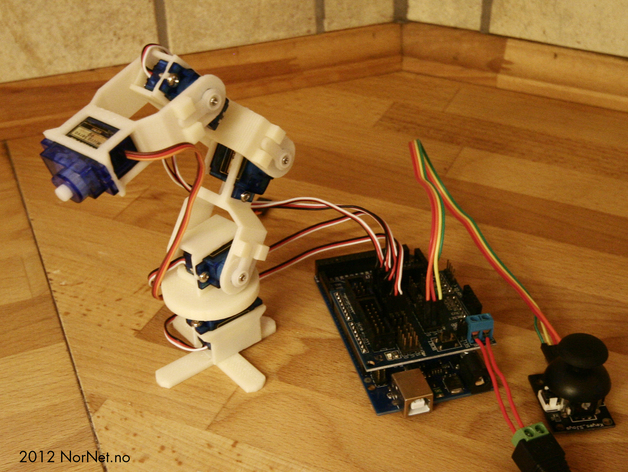
\includegraphics[width=0.45\linewidth]{servo-arm}
    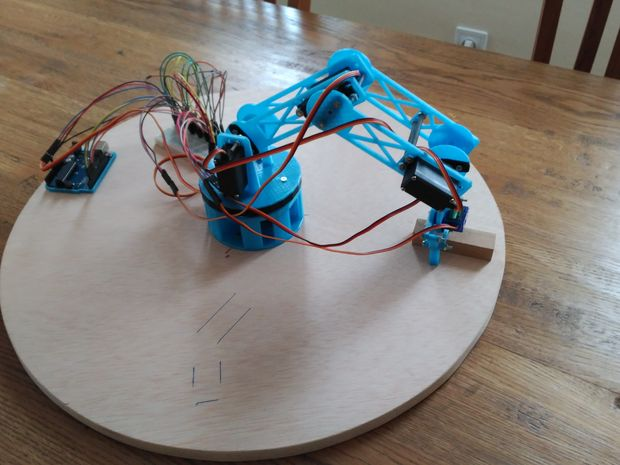
\includegraphics[width=0.45\linewidth]{servo-arm2}
    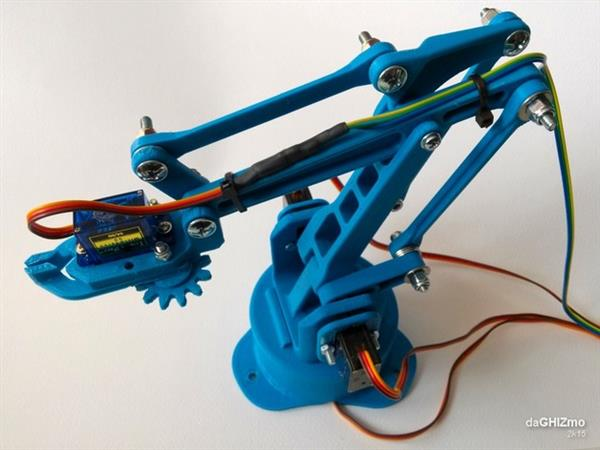
\includegraphics[width=0.45\linewidth]{servo-arm3}
    \caption{Three examples of 3D printed arms. The first one has 5 degrees of
    freedom, the second one 4 DoFs, the last one 3 DoFs.}
    \label{}
\end{figure}


\note{
    As for previous lab, you are expected to work in pairs. We only have
    enough servo-motors kits for 25 groups. \textbf{If you are not yet in a group,
    please form a pair today}.
}

Each group will be given a servo-motor kit with 2 RC mini-servos. This allows
everyone to build a robot arm with 2 degrees of freedom.

\more{
    If you wish, you can create a design with additional degrees of freedom.
    \textbf{However, you will have to source any additional actuator by
    yourselves}. Small servo-motors or stepper motors can be found online for less than 5 pounds.
}

\textbf{Working plan}

\begin{itemize}
    \item \textbf{This week}:  control of two servo-motors with the Arduino; use of 
        potentiometers to control them
    \item \textbf{Week 2}: Tutorial led by Jake on 3D design for effective 3D printing
    \item \textbf{Week 3}: Design of the arm continued; arm assembly
    \item \textbf{Week 4}: ROS on Arduino; control of the servo using ROS
    \item \textbf{Week 5}: 3D model of the arm, visualisation of the arm in RViz
    \item \textbf{Week 6}: Finalisation of arms; if time permit, 3D motion
        planning
\end{itemize}


\begin{figure}[h!]
    \centering
    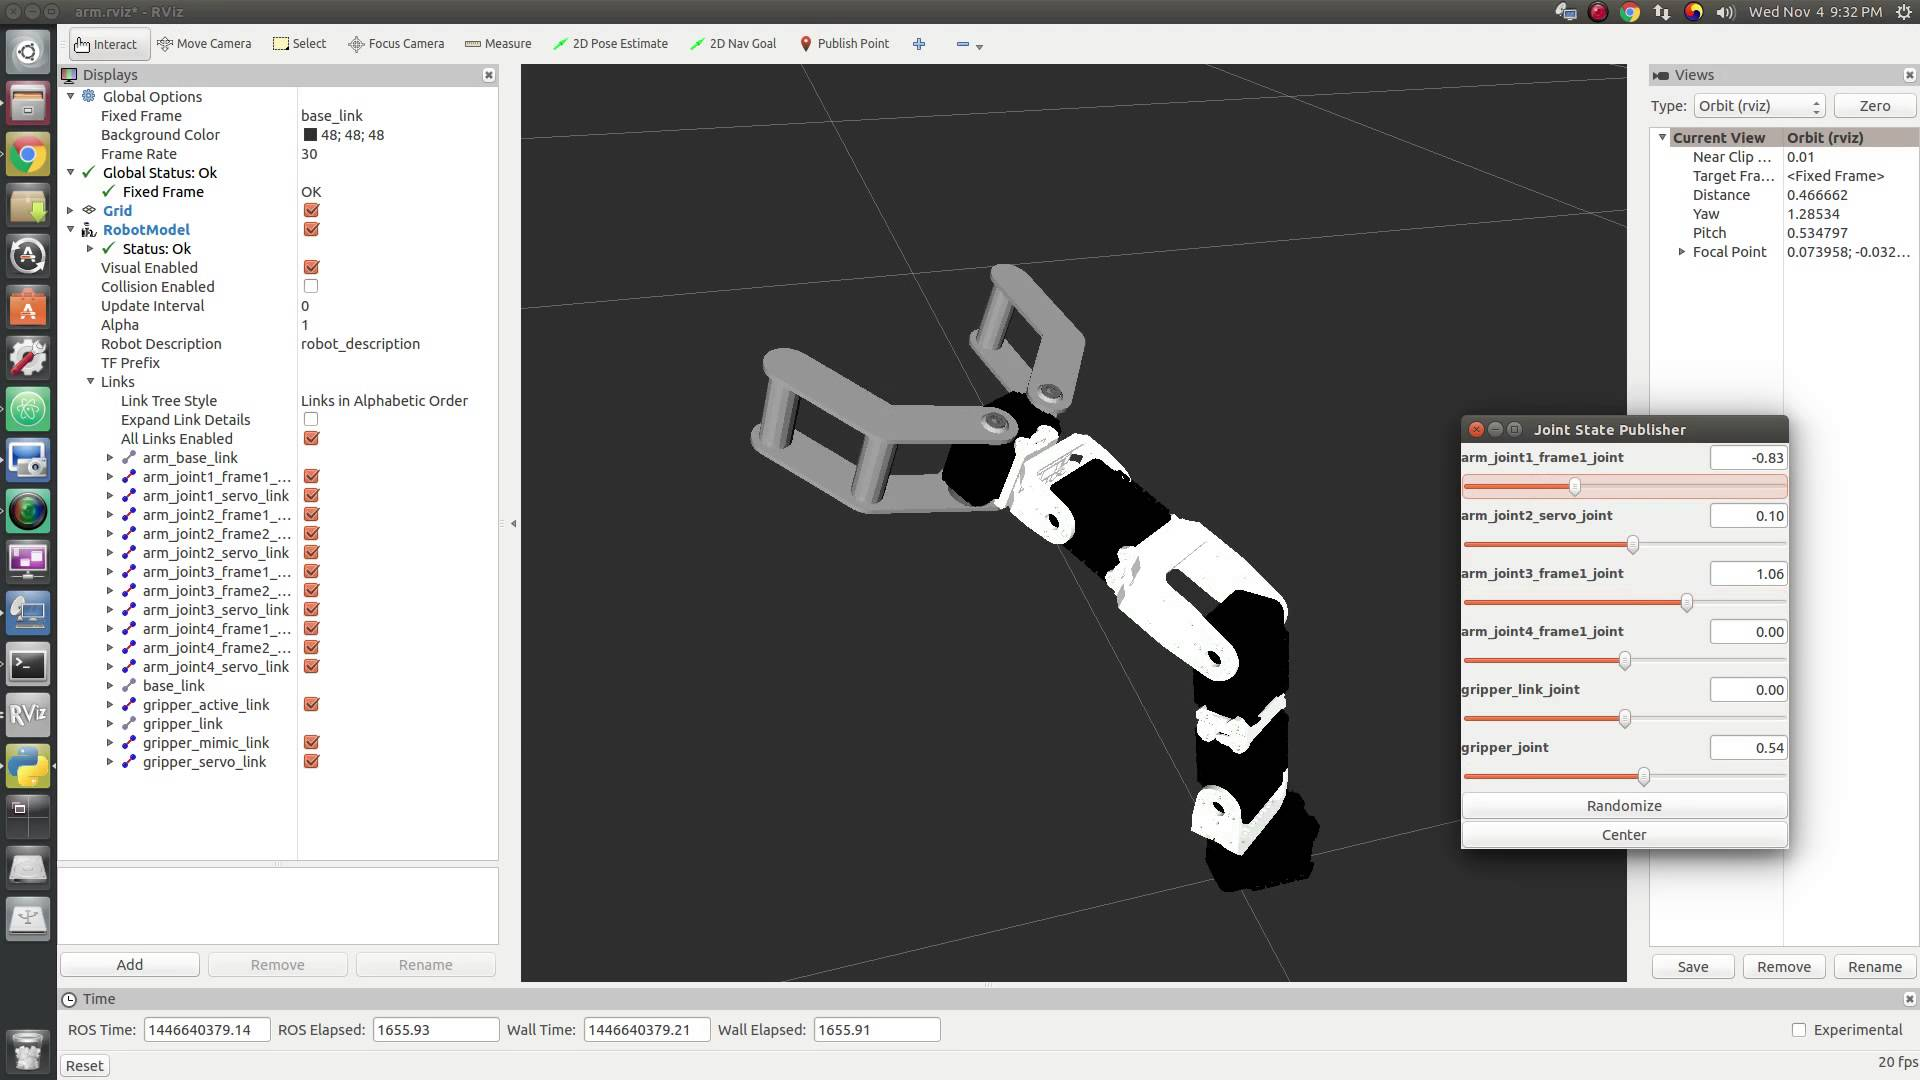
\includegraphics[width=0.9\linewidth]{servo-rviz}
    \caption{Later during the project, you will create a 3D interface to control
    your arm, using the standard ROS tools like RViz, pictured here.}
    \label{}
\end{figure}

\part{Arduino RC servo control}

The RC servomotor (Fig. \ref{servo}) is a unit consisting of a small electric
motor driving a gear train. It often uses a potentiometer to measure
angular position measurement. Often such a unit is small and cheap
although more expensive designs using metal gears and digital control
circuitry are also available. You will use such digital servo-motors in ROCO224,
next semester.

\begin{figure}[h!]
    \centering
    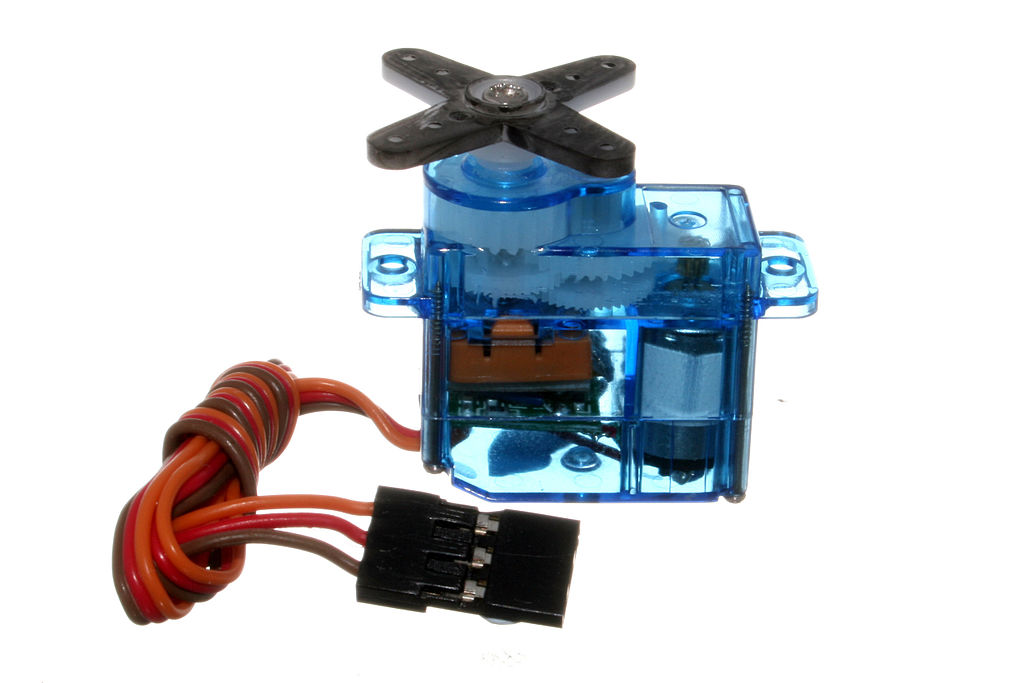
\includegraphics[width=0.6\linewidth]{figs/servo1}
    \caption{Micro-servo motor}
    \label{servo}
\end{figure}


The RC servo generally incorporates circuitry that implements position
feedback control (Fig. \ref{closedloop}). Output position compared to the commanded
target position. This gives rise to error signal. The error drives the
electric motor in appropriate direction. When it becomes zero the servo
stops moving and reaches equilibrium. A RC position servomotor usually
sets output target angle as specified by control pulse width as show in
Fig. \ref{pwm}.

\begin{figure}[h!]
    \centering
    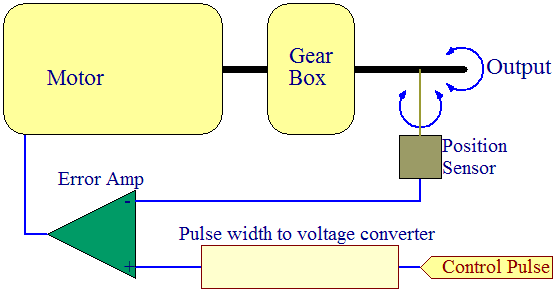
\includegraphics[width=0.6\linewidth]{figs/servo2}
    \caption{RC servo control showing feedback pathways}
    \label{closedloop}
\end{figure}

A RC servomotor typically has three connections:

\begin{itemize}
    \item Normally the black wire is ground, the red wire is connected to
        $V_{ref}$ (5V)
    and the white (or yellow) wire is the control pulse input.
\item If this is not the case on your servo, check its datasheet
\item You will need pins to connect the female plug to the female Arduino
  outputs
\end{itemize}

\begin{figure}[h!]
    \centering
    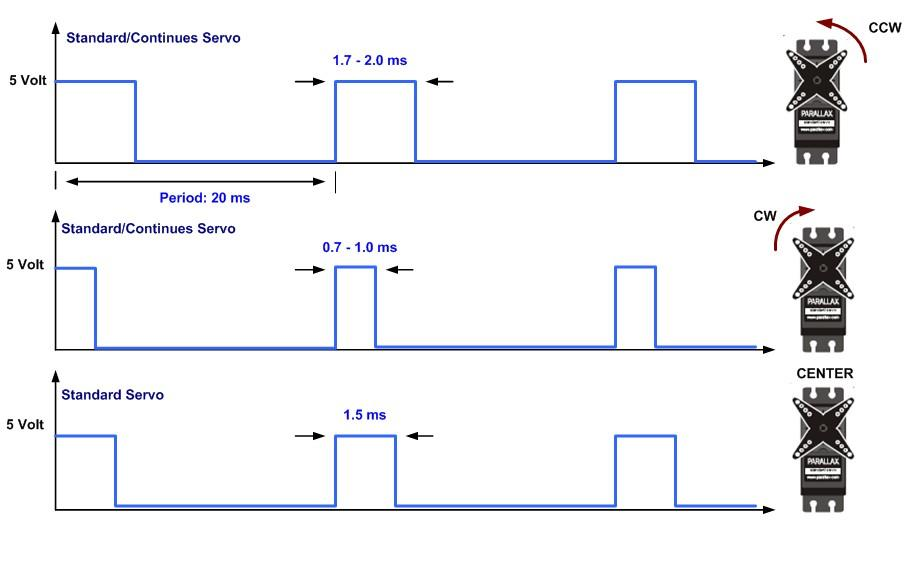
\includegraphics[width=0.9\linewidth]{figs/servo-pwm}
    \caption{RC servo operation by pulse width control}
    \label{pwm}
\end{figure}

\step{Control an RC servo}

\begin{enumerate}
\item Attach the RC servo power connections to the Arduino power output pins
\item Attach the control input to a PWM output pin on the Arduino (\eg
  port 9)
\item Write a simple program that runs the servo to generate an output
  movement back and forward over its entire range so its movement
  follows a low frequency sine wave of frequency around 0.2Hz

\end{enumerate}

\step{Control the servo with a potentiometer}

\begin{enumerate}
    \item Wire the provided potentiometer to one of the Arduino analog port.
        Write a program that reads the value of the potentiometer and writes it
        onto the serial port.
    \item Use the potentiometer to rotate the servo-motor.
\end{enumerate}

\step{A robot arm mock-up}

\begin{enumerate}
    \item Using pieces of cardboard, create an arm and attach it to the motor
        shaft (you can draw inspiration from the picture below, or come up with
        your own ideas)
    \item Estimate the torque of the servo-motor by hanging a fixed mass to the
        arm, at increasing distance of the motor shaft. Document the process,
        and check your estimate using the servo-motor datasheet (you can find it
        easily online)
    \item Modify your arm to insert the second servo motor
    \item Write a program that control both servos with the two provided
        potentiometers.
\end{enumerate}

\begin{figure}[h!]
    \centering
    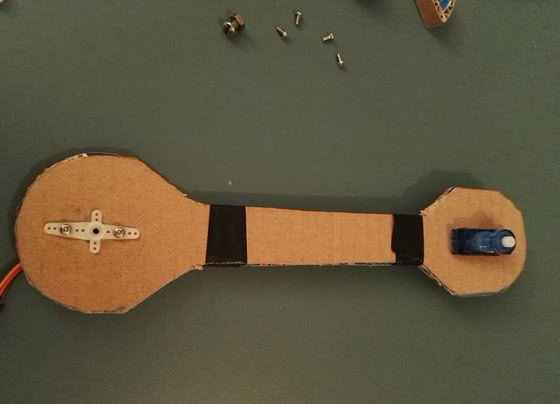
\includegraphics[width=0.9\linewidth]{figs/arm-cardboard}
    \caption{A possible assembly of 2 servos onto a cardboard arm. Taken from
    \url{http://www.instructables.com/id/CARDBIRD-the-Cardboard-Robotic-Arm/}}
    \label{}
\end{figure}




\note{
Document your findings with photographs and a short video of RC servo
operation.
}



\end{document}



